% The metal–oxide–semiconductor field-effect transistor, or MOSFET for short, is the basic building block of all modern electronics.
% It is also the most frequently manufactured device in history, with close to 10^23 MOSFETs produced since 1960.
% This compact transistor has been miniaturized and mass-produced into oblivion. During this process, it revolutionized the world economy and triggered our ascent into the information age.

\documentclass[tikz, border=5pt]{standalone}

\usetikzlibrary{patterns}

\begin{document}

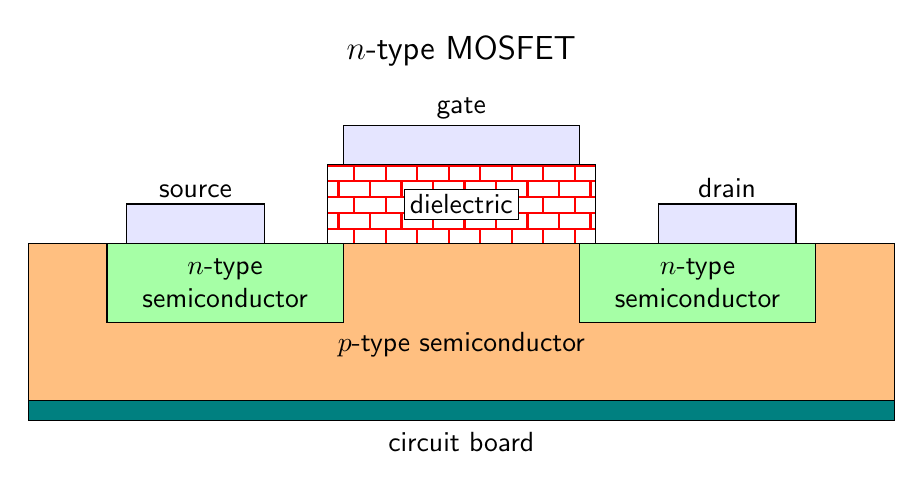
\begin{tikzpicture}[font=\sffamily]
\draw[fill = teal] (0,0) rectangle (11,-0.25) node[below=1ex, midway] {circuit board};
\draw[fill=orange!50] (0,0) rectangle (11,2) node [below,midway] {$p$-type semiconductor};
\draw[pattern=bricks, pattern color=red] (4-0.2,2) rectangle (7+0.2,3) node[midway, fill=white, inner sep=2pt, draw, ultra thin] {dielectric};
\draw[fill=blue!10] (4,3) rectangle (7,3.5) node[above=6pt, midway] {gate};
\draw[fill=blue!10] (1.25,2) rectangle (3,2.5) node[above=6pt, midway] {source};
\draw[fill=blue!10] (8,2) rectangle (9.75,2.5) node[above=6pt, midway] {drain};
\foreach \x in {1,7} {
  \filldraw[fill=green!35] (\x,1) rectangle +(3,1) node[midway, align=center] {$n$-type\\semiconductor};
}

\node[above=1ex] at (current bounding box.north) {\large $n$-type MOSFET};
\end{tikzpicture}
\end{document}
